% A workaround to allow relative paths in included subfiles
% that are to be compiled separately
% See https://tex.stackexchange.com/questions/153312/subfiles-inside-a-subfile-using-relative-paths
\providecommand{\main}{..}
\documentclass[\main/thesis.tex]{subfiles}

\begin{document}

\chapter{Results}

We created several graphs from the raw data to showcase how the two models perform for the various GLUE tasks. 

The graphs are based on the average and standard deviations across the 5 runs we 
conducted for each of the GLUE tasks. 

\section{CoLA Results}\label{sec:cola_results}

We will start with the CoLA results where we saw the most different between the two models. 

The Corpus of Linguistic Acceptability (CoLA) task is focused on a model's ability 
to recognize a malformed sentence (grammatically). An example of a malformed sentence that is 
part of the dataset is `Who does John visit Sally because he likes'.

CoLA comprises sentences sourced from the linguistic literature, each of which is labeled in terms of its grammatically:
\begin{itemize}
    \item \textbf{Acceptable} - The sentence is grammatically correct.
    \item \textbf{Unacceptable} - The sentence is grammatically incorrect.
\end{itemize}

This dataset provides a unique challenge as it demands models to capture deeper linguistic knowledge rather than relying on mere statistical patterns. 
Traditional metrics like accuracy are used to evaluate models on the CoLA dataset, alongside more specialized metrics like the Matthews correlation coefficient.

\begin{figure}
    % \centering
    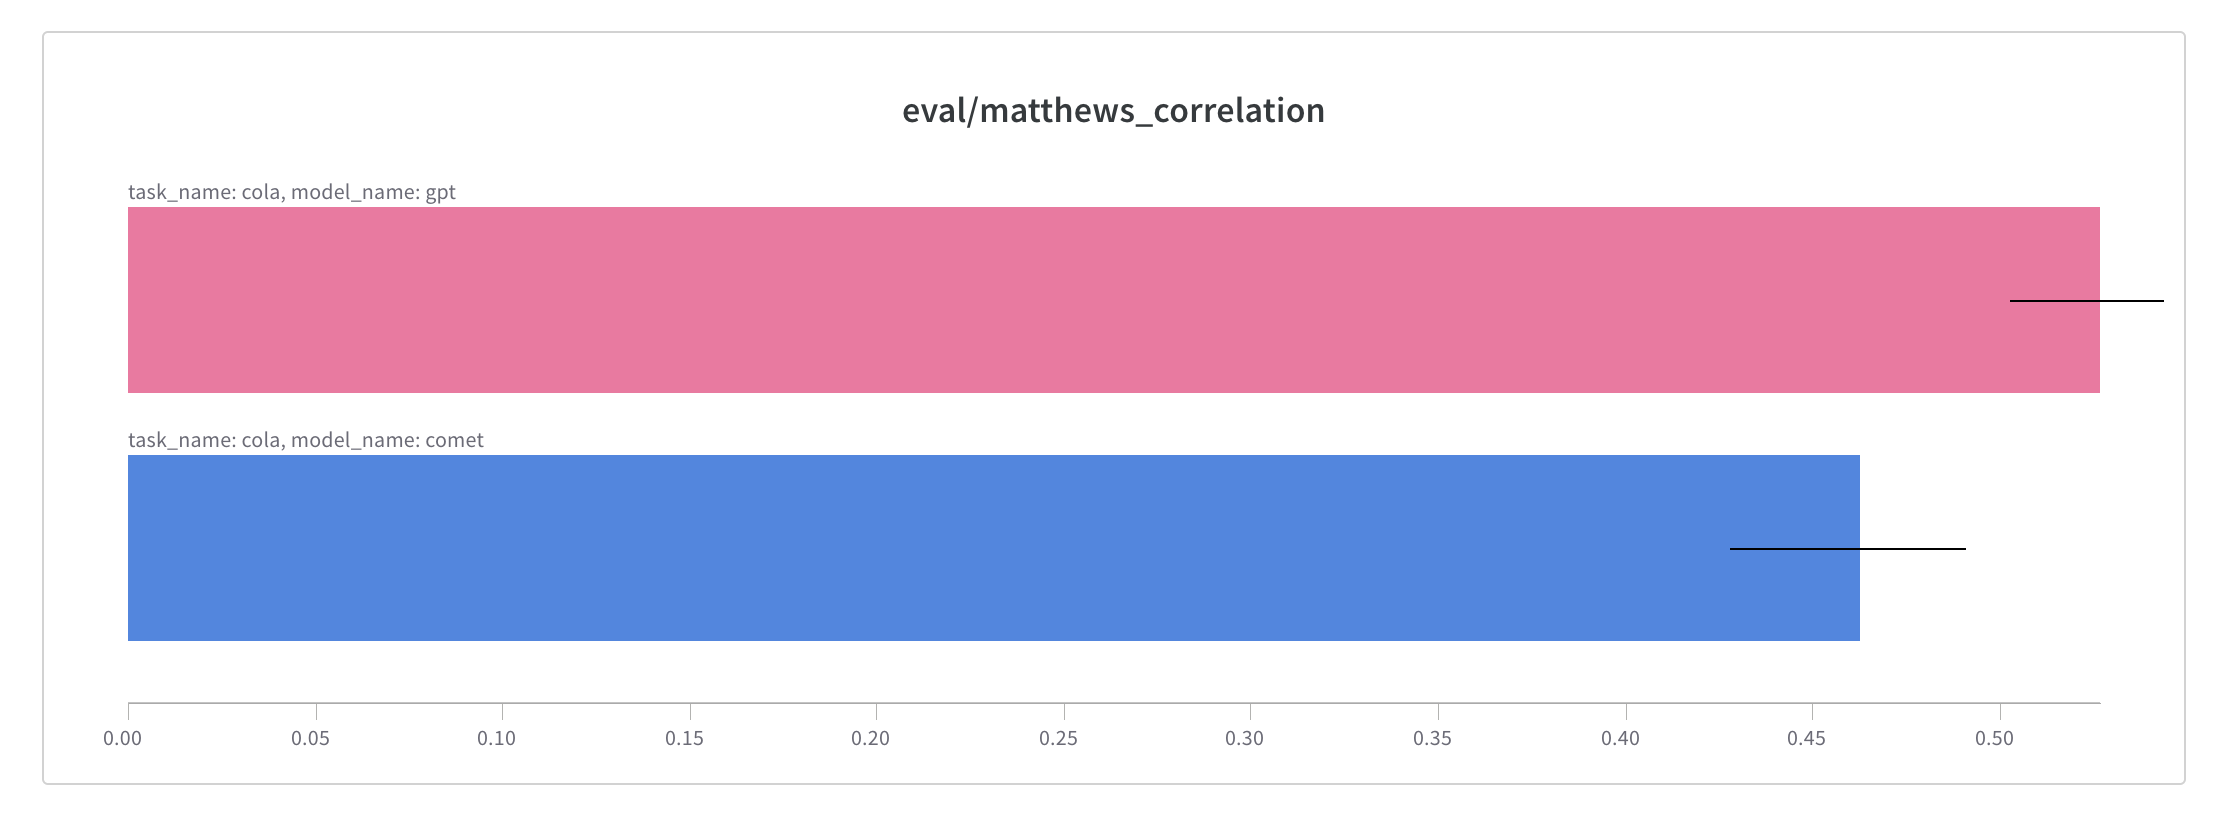
\includegraphics[keepaspectratio=true, width=0.9\textwidth]{\main/img/COLA}
    \caption[GLUE Results: CoLA] {GLUE Results: CoLA}
    \label{fig:cola_fig}
    % Put the label *after* the caption, but inside the float
\end{figure}

GPT-2 XL and COMET had  Matthews correlation coefficient of 0.53 $\pm$ 0.02 and 0.46 $\pm$ 0.02 respectively. This was markedly the largest
difference we saw between the two models for any of the GLUE tasks. 

In order to understand how the models differed, we analyzed the results from the COLA task further. 
We used the validation subset and made predictions on it. Then we compared the predictions between
the two models and the ground truth. We saw that there were 160 instances from the total 
subset of 1043 instances where the two models disagreed. 

Upon Analyzing our results for the CoLA task, we noticed that the COMET 
model struggled with instances where something was happening in the past tense.

An example of this would be `There presented itself a wonderful opportunity yesterday.' 
This is supposed to be a malformed sentence. The naive GPT-2 XL model is able to 
recognize it as such but the COMET model fails to do so. 

\section{RTE Results}\label{sec:rte_results}

The second difference we noticed between the two models was on the RTE task where GPT-2 XL
 and COMET had accuracy scores of 0.773 $\pm$ 0.009 and 0.680 $\pm$ 0.1. Given that
there was a lot of variability between the runs for the COMET model, we are not conclusive
about the difference in the performance between the naive GPT-2 XL and the specialized
COMET model. 

To provide some context, Recognizing Textual Entailment (RTE) is a benchmark challenge 
that focuses on determining whether a given piece of text (the ``hypothesis'') can be inferred or 
entailed by another piece of text (the ``text'' or ``premise''). Typically, for any given pair of texts, 
the model is required to decide among three possible relations:

\begin{enumerate}
    \item \textbf{Entailment}: The hypothesis is a logical consequence of the text. That is, 
    if the text is true, then the hypothesis is necessarily true as well.
    \item \textbf{Contradiction}: The hypothesis is logically inconsistent with the text. 
    This means that both cannot be true at the same time.
    \item \textbf{Neutral}: The relationship between the text and the hypothesis is neither one of entailment nor contradiction. 
    The truth of the text does not guarantee the truth or falsity of the hypothesis.
\end{enumerate}

For example:
\begin{itemize}
    \item Text: ``The cat is sleeping on the sofa.''
    \begin{itemize}
        \item Hypothesis 1: ``There is a cat on the sofa.'' (Entailment)
        \item Hypothesis 2: ``The cat is playing outside.'' (Contradiction)
        \item Hypothesis 3: ``The sofa is blue.'' (Neutral)
    \end{itemize}
\end{itemize}

RTE has been an important task in NLP because it captures a fundamental aspect of human language understanding. 

\begin{figure}
    % \centering
    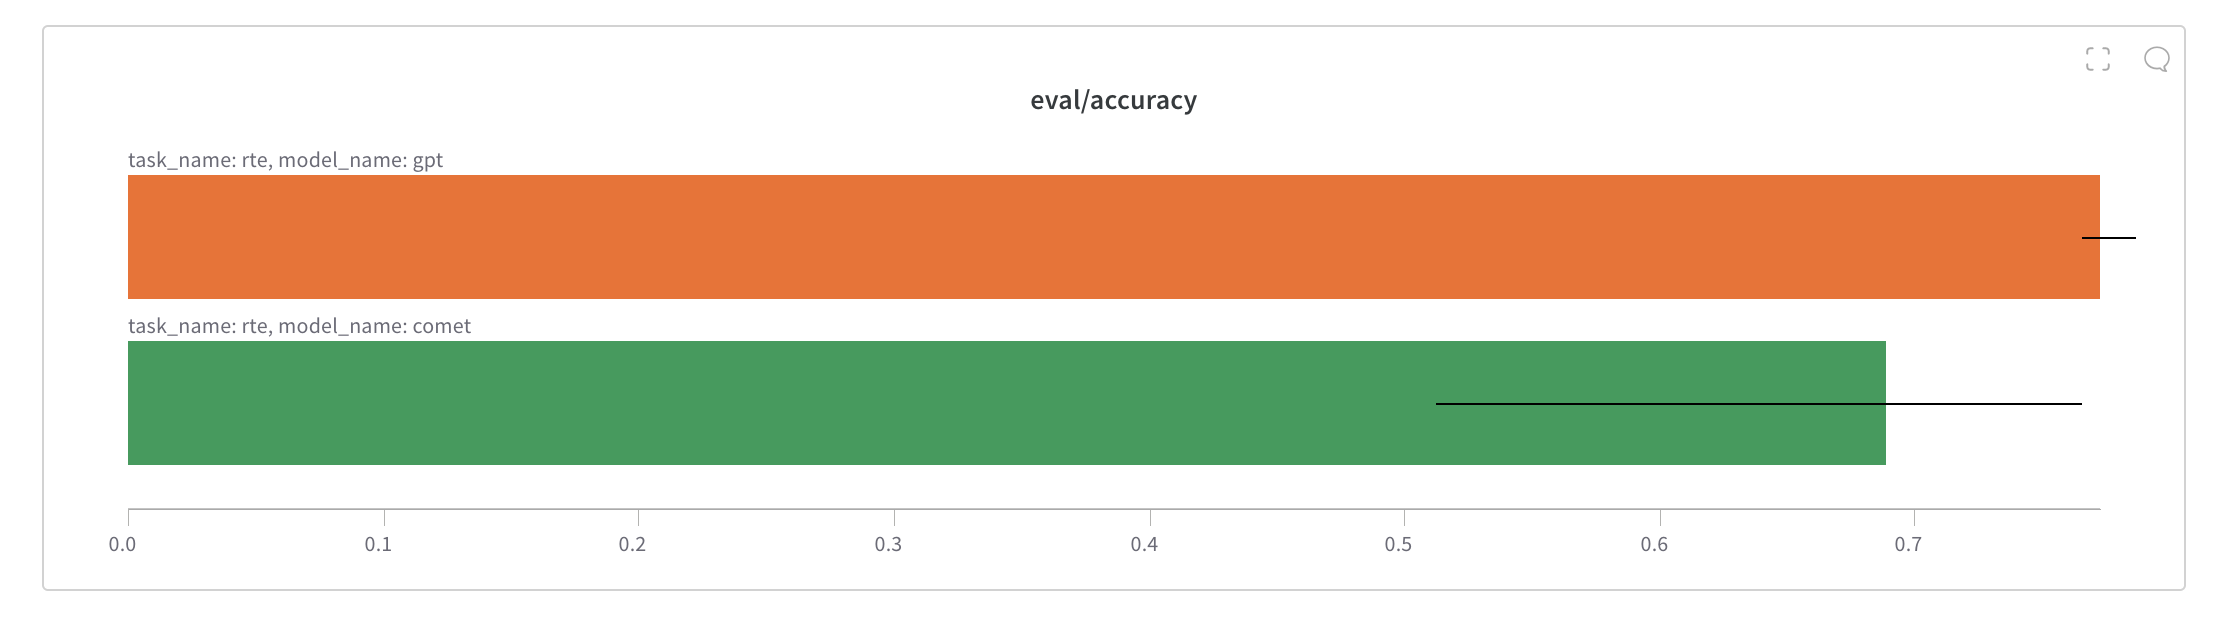
\includegraphics[keepaspectratio=true, width=0.9\textwidth]{\main/img/RTE}
    \caption[GLUE Results: RTE] {GLUE Results: RTE}
    \label{fig:rte_fig}
    % Put the label *after* the caption, but inside the float
\end{figure}

Upon analyzing the individual predictions between the models for the validation dataset,
we could not find a discernible pattern such as the one we saw in CoLA.
As such, we conclude that this difference in performance may just be statistical noise. 

For the rest of the tasks in the GLUE dataset, we have provided a summary figure. It indicates 
that there was not a very large difference in the performance of the two models. 

\begin{figure}
    % \centering
    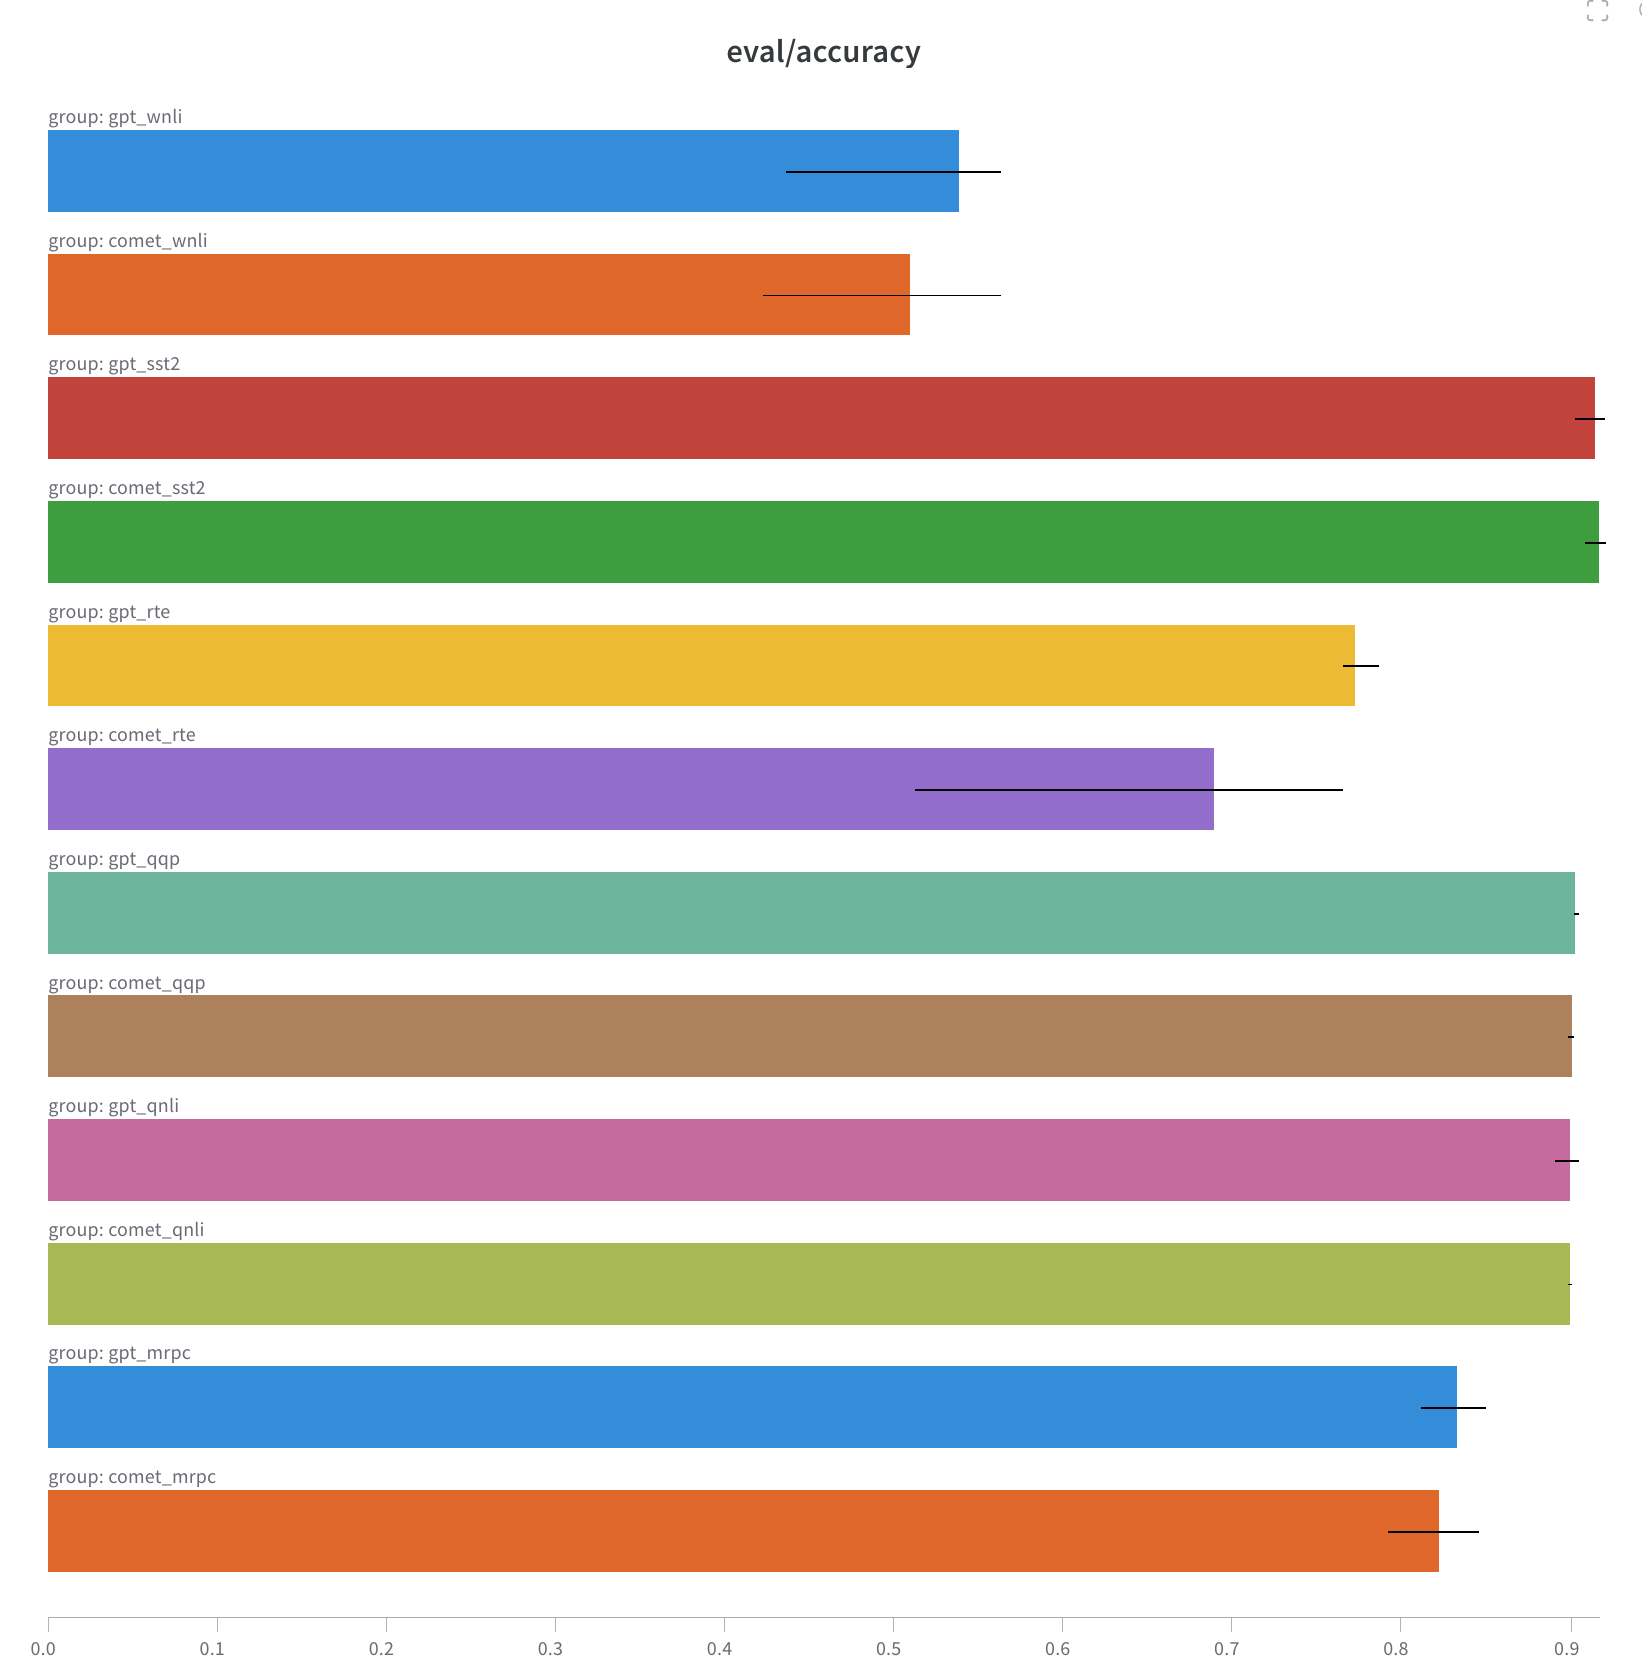
\includegraphics[keepaspectratio=true, width=0.9\textwidth]{\main/img/SUMMARY}
    \caption[GLUE Results: Summary] {GLUE Results: Summary}
    \label{fig:rte_fig}
    % Put the label *after* the caption, but inside the float
\end{figure}

\end{document}